\documentclass{article}

\usepackage{microtype}
\usepackage{graphicx}
\usepackage{booktabs}
\usepackage{hyperref}
\usepackage{tikz}
\usetikzlibrary{arrows.meta,positioning,fit,calc}

\newcommand{\theHalgorithm}{\arabic{algorithm}}
\usepackage[preprint]{icml2026}
\usepackage{amsmath}
\usepackage{amssymb}
\usepackage{url}

\icmltitlerunning{AI Research Writing Skill}

\begin{document}

\twocolumn[
\icmltitle{AI Research Writing Skill: Claim-Evidence Engineering for Agentic Research Paper Generation}

\begin{icmlauthorlist}
  \icmlauthor{Example Paper Package}{demo}
\end{icmlauthorlist}

\icmlaffiliation{demo}{Demonstration Artifact}
\icmlcorrespondingauthor{Example Maintainer}{example@example.com}
\icmlkeywords{Machine Learning, Research Writing, AI Agents, LaTeX, Reproducibility}

\vskip 0.3in
]

\printAffiliationsAndNotice{}

\begin{abstract}
AI agents can draft fluent research prose, but scientific paper writing also requires evidence discipline: claims must be traceable, citations must be verified, figures and tables must become concrete assets, and submission readiness must be checked. This example paper describes AI Research Writing Skill, a portable agent skill for turning ML/AI research repositories into auditable paper packages. The contribution is a workflow contract rather than a benchmarked model: it specifies how an agent should inventory a repository, construct a paper story, maintain a claim-evidence map, verify citations, design figures and tables, run reviewer-style checks, and compile a build-ready LaTeX package. We use the repository itself as the case study. The resulting artifact demonstrates how a single canonical skill entrypoint, modular references, venue templates, deterministic helper scripts, generated concept figures, and explicit risk records can coordinate an end-to-end repo-to-paper workflow without claiming empirical performance improvements.
\end{abstract}

\begin{figure*}[t]
\centering
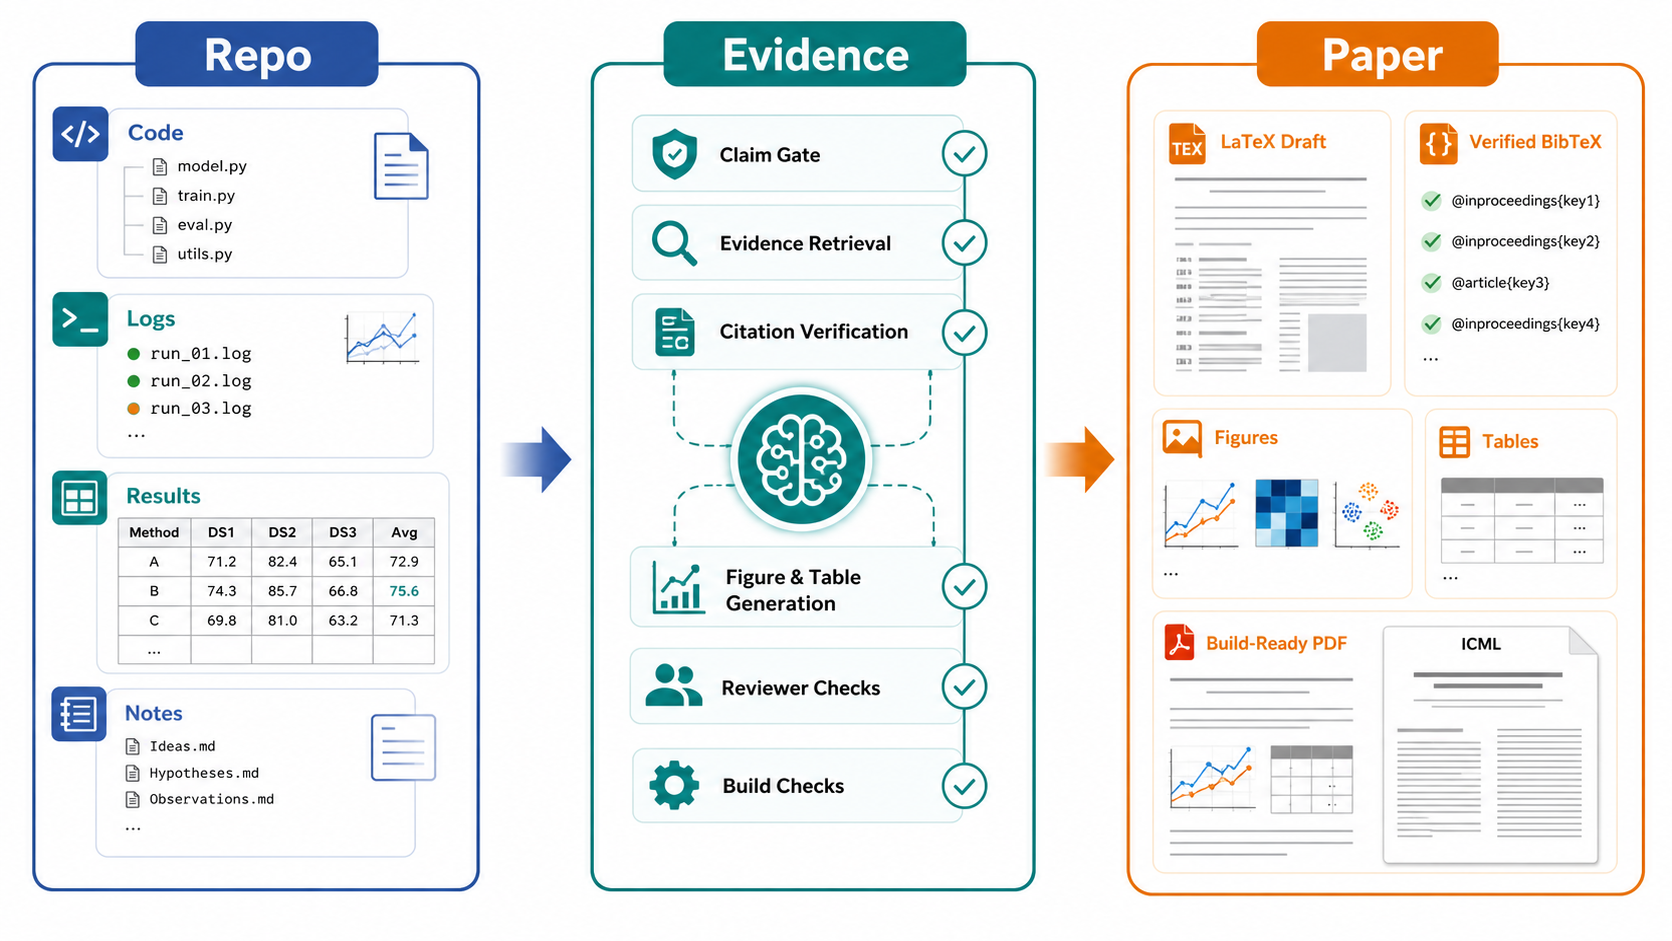
\includegraphics[width=\textwidth]{figures/teaser_imagegen.png}
\caption{Teaser generated with image generation. The project reframes agentic paper writing as a transformation from repository evidence to a build-ready paper package.}
\label{fig:teaser}
\end{figure*}

\section{Introduction}

Large language models and coding agents can accelerate research writing, but prose generation alone is a poor unit of scientific progress. A paper draft is only useful if the reader can inspect which results support which claims, which citations support which background statements, which figures carry conceptual versus numerical evidence, and which artifacts are ready for submission. A fluent draft that cannot be traced back to code, logs, notes, or verified literature is difficult to review and risky to submit.

This problem is especially visible in ML and AI projects, where a paper often emerges from a live repository rather than from a static manuscript. The relevant evidence may be distributed across implementation files, experiment logs, result tables, plotting scripts, meeting notes, and venue-specific templates. The writing agent therefore needs more than paragraph-level style guidance: it needs a workflow for deciding what can be claimed, what must be weakened, what citations must be checked, and what files must be produced before the paper package can be considered complete.

AI Research Writing Skill addresses this need by treating paper generation as claim-evidence engineering. The skill is designed as a portable instruction package with a single canonical entrypoint, \texttt{SKILL.md}. Instead of promising autonomous scientific discovery, it constrains an agent to produce auditable artifacts: a repository inventory, paper story, claim-evidence map, citation verification record, figure and table assets, reviewer-style risk analysis, and build notes. These artifacts make the agent's intermediate decisions visible to the human author.

The project builds on a growing ecosystem of research-writing and research-agent resources, including compact paper-writing skills~\cite{masterCaiResearchPaperWritingSkills}, broad multi-platform writing assistants~\cite{normanBuryResearchWritingSkill}, general AI research skill libraries~\cite{orchestraResearchAISkills}, Nature-style publication workflows~\cite{yuanNatureSkills}, and publication figure resources~\cite{chenFigures4Papers}. Its narrower focus is the ML/AI repository-to-paper setting: an agent works inside a codebase, inspects notes and results, and produces a paper package with explicit evidence boundaries.

This paper is itself an example output of the skill. We do not report benchmark scores, user-study results, or acceptance-rate improvements. Instead, we present a system artifact and a repository-backed case study. The claims in this paper are intentionally structural: they describe what the repository contains, how the workflow is organized, and what checks are run. This makes the example useful as a demonstration while avoiding unsupported claims about downstream writing quality.

The main contributions are:
\begin{itemize}
  \item a claim-evidence-engineering formulation for agentic research paper generation;
  \item a portable single-entrypoint skill design that lets different agents load the same root contract;
  \item an artifact contract for full-paper work, covering story, evidence, literature, figures, review, and build readiness;
  \item an ICML-style example paper package with generated overview figures, LaTeX tables, verified citations, and a compiled PDF.
\end{itemize}

\section{Problem Setting}

We consider the setting where a researcher has an ML/AI repository and wants an agent to help produce a conference-style paper package. The input may include source code, notes, partial experimental results, venue templates, related-project links, and informal claims. The output should not be only prose. It should include a manuscript plus supporting files that explain how the prose was derived and what remains uncertain.

This setting has three constraints. First, evidence is heterogeneous. A claim about an algorithm may come from code or method notes, while a claim about performance must come from logs, tables, or scripts, and a claim about prior work must be backed by verified citation metadata. Second, the agent's decisions should be inspectable. If the agent decides not to claim superiority, or weakens a statement because evidence is missing, that decision should be recorded. Third, paper readiness is operational. A draft is not ready merely because text exists; citations, figures, tables, checklists, and LaTeX build status also matter.

We define the core task as producing an auditable paper package. An auditable package contains the manuscript, but also the intermediate artifacts needed to review claim support, citation status, figure provenance, and build readiness. This framing turns paper writing from a single generation step into a sequence of bounded transformations.

\section{System Design}

Figure~\ref{fig:method-overview} summarizes the workflow. The root skill contract defines operating modes for full-paper drafting, story building, section writing, figures, citations, reviewer checks, submission, and automation. References are loaded progressively so that a task uses the narrow guidance it needs rather than the entire documentation tree.

\begin{figure*}[t]
\centering
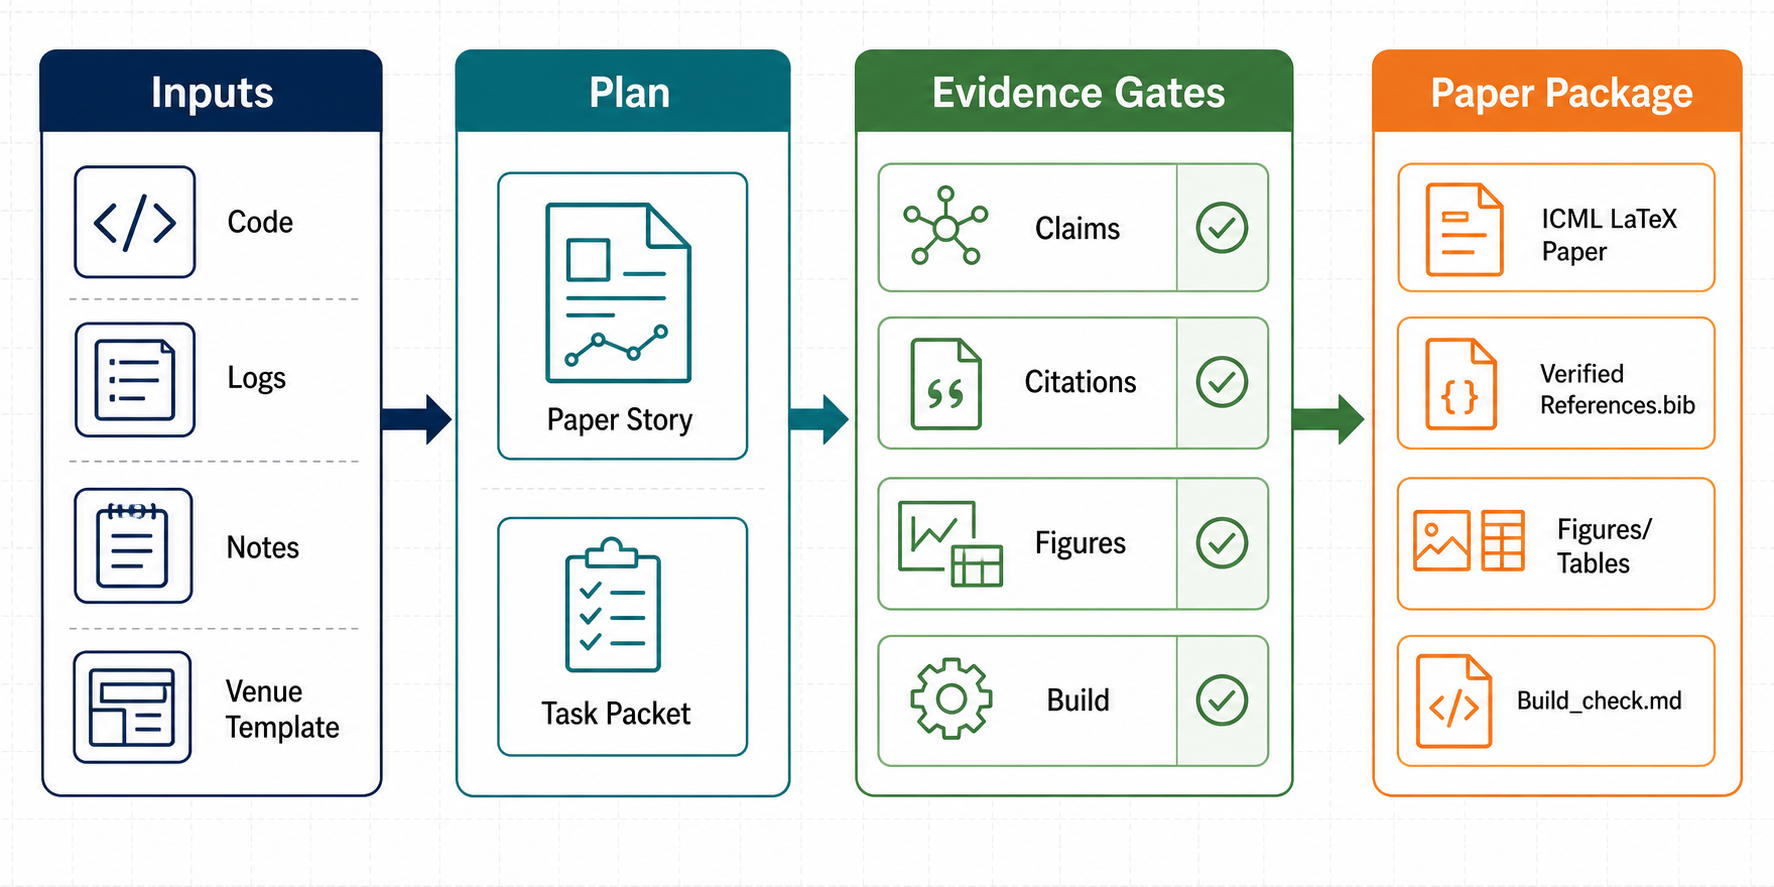
\includegraphics[width=\textwidth]{figures/overview_imagegen.png}
\caption{Method overview generated with image generation. AI Research Writing Skill coordinates repository inputs, planning artifacts, evidence gates, and paper-package outputs. The figure is conceptual and is not used as numerical evidence.}
\label{fig:method-overview}
\end{figure*}

The design has four main principles. First, strong claims must be backed by local repository evidence, experiment artifacts, notes, or verified citations. Second, generated numeric evidence is disallowed: image models may create conceptual diagrams, but result plots and tables must be produced from deterministic data or scripts. Third, the output should be durable. Story files, claim maps, citation verification notes, figure plans, generated assets, and build checks are written into the target paper repository. Fourth, completion claims require verification or explicit blockers.

The root \texttt{SKILL.md} acts as the canonical contract. It defines the mandate, operating modes, loading strategy, evidence policy, non-negotiable gates, and output discipline. Supporting references provide more detailed guidance for particular tasks such as citation verification, figure planning, reviewer self-review, and submission packaging. This separation keeps installation simple while preserving depth: users install or load one skill entrypoint, and the agent pulls in narrower references only when needed.

\paragraph{Artifact contract.}
For full-paper work, the skill asks the agent to maintain durable artifacts rather than relying on hidden chain-of-thought or ephemeral chat context. A typical package includes \texttt{paper\_story.md} for thesis and contribution boundaries, \texttt{claim\_evidence\_map.md} for supported and unsupported claims, \texttt{citation\_verification.md} for BibTeX provenance, \texttt{figures/figure\_plan.md} for diagram and plot intent, and \texttt{build\_check.md} for compilation status. These files create a lightweight audit trail that a human author can inspect before trusting the generated manuscript.

\paragraph{Gate structure.}
The workflow uses gates to prevent premature drafting. The story gate prevents full-paper writing before thesis and contribution boundaries are explicit. The literature gate prevents Related Work prose before positioning is recorded. The citation gate requires verified BibTeX or visible placeholders. The figure gate separates generated conceptual diagrams from deterministic numeric plots. The build gate requires compilation or a recorded blocker. In this example, the gates are visible through the surrounding markdown artifacts and validation commands.

\section{Implementation}

The implementation is intentionally repository-native. The skill does not require a service backend or a custom plugin runtime. Its main components are:
\begin{enumerate}
  \item \textbf{Canonical entrypoint}: \texttt{SKILL.md} describes the agent behavior and routes tasks to references.
  \item \textbf{Reference library}: \texttt{references/} contains focused guidance for workflow, writing, citations, figures, venues, review, task management, and packaging.
  \item \textbf{Template collection}: \texttt{templates/} provides convenience LaTeX starters for major ML/AI venue families.
  \item \textbf{Deterministic helper scripts}: \texttt{scripts/} contains static checks for claims, citations, unresolved markers, build logs, camera-ready readiness, and table generation.
  \item \textbf{Example package}: \texttt{examples/} demonstrates the full workflow on this repository itself.
\end{enumerate}

This design trades platform-specific automation for portability. Any capable agent can be instructed to load the root skill file and then inspect the supporting directories. The README therefore recommends agent-assisted installation rather than maintaining multiple host-specific plugin wrappers.

\section{Repository Evidence}

Table~\ref{tab:repository-evidence} summarizes local evidence used for this example paper. The repository includes venue template directories for major ML/AI conference families, top-level references for writing and submission workflows, helper scripts for static checks and table generation, and a portable single-entrypoint design centered on the root skill file.

\begin{table*}[t]
\centering
\begin{tabular}{p{0.28\linewidth}p{0.18\linewidth}p{0.44\linewidth}}
\toprule
Repository evidence & Count / scope & Paper claim supported \\
\midrule
Venue template directories & 9 & Multi-venue ML/AI template support \\
Top-level reference files & 21 & Modular workflow guidance \\
Top-level script files & 8 & Deterministic quality checks and helpers \\
Cross-platform entrypoints & 8 groups & Claude, Cursor, Codex, Gemini, OpenCode support \\
\bottomrule
\end{tabular}
\caption{Repository evidence used by the example paper. Counts are derived from the local project tree at the time this example was created.}
\label{tab:repository-evidence}
\end{table*}


These counts are not performance metrics. They support only structural claims about what the repository contains. They do not establish that the skill improves writing quality, acceptance probability, or agent reliability.

\section{Case Study: Writing This Paper}

The example directory instantiates the workflow on the skill repository itself. The initial prompt asks the agent to treat \texttt{ai-research-writing-skill} as the research artifact, inspect the repository, avoid invented performance numbers, and produce an ICML-style paper package. The generated package includes a story file, claim-evidence map, citation verification record, literature positioning notes, LaTeX source, tables, generated overview images, and a build check.

The story artifact defines the thesis as a claim-evidence-engineering workflow for agents working inside ML/AI repositories. The claim map separates supported structural claims from unsupported claims. For example, it permits claims about repository contents, helper scripts, template coverage, and workflow design, but rejects claims about guaranteed acceptance, correctness, or superiority over related tools. This distinction directly shapes the paper text: the abstract and introduction describe the system and case study, but avoid empirical performance claims.

The figure workflow uses generated images for conceptual communication and deterministic LaTeX tables for repository evidence. The teaser and method overview are therefore illustrations of the process, while Table~\ref{tab:repository-evidence} carries count-based repository evidence. This separation is important because generated images can clarify architecture but cannot create scientific measurements.

The build workflow compiles the paper with the bundled ICML-style files and records warnings in \texttt{build\_check.md}. The resulting PDF is included in the repository so readers can inspect the output quality directly. The build record also lists residual risks, including the absence of benchmark evidence and the need to verify official venue requirements before any real submission.

\section{Quality Checks}

The repository includes helper scripts that operationalize part of the workflow. Citation checks scan LaTeX citation keys against the BibTeX file. Marker checks look for unresolved notes in manuscript artifacts. A research quality gate scans for common unresolved placeholders and missing package components. Build-log parsing and camera-ready checks provide additional submission-oriented signals.

These scripts are deliberately modest. They do not prove semantic correctness, validate every citation claim, or guarantee venue compliance. Their role is to catch mechanical failures and force unresolved risks into visible records. In the workflow, script output is paired with human review and reviewer-style critique rather than treated as an oracle.

\section{Related Projects}

Table~\ref{tab:related-projects} positions AI Research Writing Skill against neighboring open-source projects. The comparison is intended to clarify scope rather than rank projects.

\begin{table*}[t]
\centering
\begin{tabular}{p{0.28\linewidth}p{0.30\linewidth}p{0.34\linewidth}}
\toprule
Project & Main focus & Distinction of this project \\
\midrule
Research-Paper-Writing-Skills & ML/CV/NLP writing skills & Adds repo-to-paper artifacts and checks \\
research-writing-skill & General research writing & Narrows to AI conference paper packages \\
AI-research-SKILLs & Broad AI research skills & Focuses on paper execution and readiness \\
nature-skills & Nature-style publication workflow & Targets ML/AI conference workflows \\
figures4papers & Publication figure scripts & Connects figures to claims and LaTeX checks \\
\bottomrule
\end{tabular}
\caption{Positioning against related open-source projects.}
\label{tab:related-projects}
\end{table*}


The key distinction is operational depth in one vertical. Instead of serving as a general thesis assistant or a figure-only resource, this project specifies a complete paper package contract for ML/AI agents working over real research repositories.

\section{Limitations}

This example paper has important limitations. It does not benchmark the skill against other writing systems. It does not show user-study evidence. It does not prove that generated papers are correct, useful, or publishable. The repository inventory establishes only that certain files and workflows exist, not that they improve author productivity or paper quality.

The workflow also depends on the agent and user applying the gates faithfully. A careless agent could still overstate a claim, cite an irrelevant source, or ignore a build warning. The skill reduces this risk by requiring explicit artifacts and checks, but it cannot eliminate the need for human scientific judgment.

Finally, venue templates bundled in the repository are convenience copies. Official author instructions, page limits, checklist requirements, anonymity rules, and camera-ready policies can change. Any real submission must therefore verify venue requirements against official sources before use.

\section{Conclusion}

AI Research Writing Skill reframes agentic paper drafting as a claim-evidence-engineering process. By combining repository inspection, durable artifact contracts, verified citation practices, figure and table assets, a portable root skill entrypoint, reviewer-style risk analysis, and build-readiness checks, it offers a concrete workflow for turning ML/AI research repositories into auditable paper drafts. The example paper demonstrates the intended output style: not a claim of autonomous scientific correctness, but a transparent package whose claims, evidence, assets, and remaining risks can be inspected.

\bibliographystyle{icml2026}
\bibliography{references}

\end{document}
